% Compile on Overleaf (IEEEtran is built in). Upload main.tex + refs.bib, set compiler to pdfLaTeX.
% Sections 4 (Method) and 5 (Experimental Setup) are drafted from the code at the commit noted in
% \codecommit. Everything marked \tbd{...} is filled in after the GPU runs. \todo{...} = open decision.
\documentclass[conference]{IEEEtran}
\usepackage{iftex}
\ifPDFTeX
  \usepackage[T1]{fontenc}   % pdfLaTeX (Overleaf): IEEEtran's Times
\else
  \usepackage{fontspec}       % XeTeX (local Tectonic builds): same Times look
  \setmainfont{texgyretermes}[Extension=.otf, UprightFont=*-regular, BoldFont=*-bold,
    ItalicFont=*-italic, BoldItalicFont=*-bolditalic]
\fi
\usepackage{amsmath,amssymb}
\usepackage{booktabs}
\usepackage{graphicx}
\usepackage{xcolor}
\usepackage{url}
\usepackage{cite}

\newcommand{\tbd}[1]{\textcolor{red}{[TBD: #1]}}
\newcommand{\todo}[1]{\textcolor{orange}{[TODO: #1]}}
\newcommand{\codecommit}{\texttt{\tbd{commit}}}
\newcommand{\RR}{\mathrm{RR}}
\newcommand{\PSI}{\mathrm{PSI}}

\begin{document}

\title{Where Does a Wrong Step Hurt? Error Position, Remaining Steps, and Thinking Mode in Multi-Hop Reasoning}

\author{\IEEEauthorblockN{\tbd{Authors}}
\IEEEauthorblockA{Dept. of CSE (AI\&ML), M.S. Ramaiah Institute of Technology, Bengaluru, India}}

\maketitle

\begin{abstract}
When a language model makes a wrong step in a chain of reasoning, does the position of that step decide whether it recovers? Prior studies disagree, and their designs confound position with the number of steps that remain and with the final, answer-producing step. We plant errors at exact hop positions in models' own reasoning chains on 3- and 4-hop MuSiQue questions, resume generation, and measure recovery against an uncorrupted resume of the same chain. We test Qwen3-8B with thinking off and on (same weights) and Llama-3.1-8B.
Late intermediate errors are recovered less often than early ones, by 9--20 percentage points at three hops in every model and mode. For Qwen3 this is not a position effect as such. At a fixed number of remaining steps, position has no detectable effect, and the next hop catches early and late errors equally often; late errors simply leave fewer hops on which to recover. Llama shows a residual position effect.
Errors in the final hop are almost never recovered without thinking, and counting them as ``late'' would inflate the position effect 2.3--3.2-fold. Recovery is higher in thinking mode, but prefilling a hop summary inside the thinking block ends the model's deliberation, a pitfall for prefill-based studies. Almost all recoveries are silent. \tbd{one sentence on think\_trace if it works.}
\end{abstract}

\begin{IEEEkeywords}
chain-of-thought, error propagation, multi-hop question answering, reasoning models, robustness
\end{IEEEkeywords}

% ======================================================================
\section{Introduction}
Language models answer multi-step questions by chaining intermediate results, and any step can go wrong. Whether a wrong step ruins the answer depends on whether the model later notices or works around it. If errors at some positions are reliably recovered and errors at others are not, step-level verification~\cite{lightman} and checks in agent pipelines should concentrate where recovery fails. Knowing \emph{where} a wrong step hurts most therefore has practical value.

Prior studies disagree on the answer. Von Recum et al.~\cite{vonrecum} intervene in reasoning models' own chains at fixed points and find that early interventions hurt more. Jia and Mu~\cite{jiamu} perturb one step and let the model continue. They find that error propagation falls from 33.5\% for early steps to 22.5\% for late ones, but call the gradient ``partly mechanical'': earlier steps have more steps left after them, and task difficulty dominates. ASCoT~\cite{ascot} reports the opposite, \emph{late-stage fragility}, for Qwen2.5-7B on GSM8K. Its largest accuracy drops, however, come from corrupting the final step (52 points at step 4 of 4), which produces the answer directly. These designs leave three variables entangled: the position of the error, the number of steps that remain after it, and whether the corrupted step is the terminal one. All three studies also use math, science or logic tasks, whose intermediate steps have no gold values, so an injected error's position and correctness are only approximate.

We study error position in multi-hop question answering, where these variables can be controlled. Each MuSiQue~\cite{musique} question is composed of single-hop questions with gold intermediate answers. We keep items whose own chain matches the gold decomposition hop by hop, replace one hop's answer with a wrong value of the same entity type, and let the model continue from the corrupted chain. Recovery is measured against an uncorrupted resume of the same chain. Crossing chain length (3 and 4 hops) with hop position yields pairs of errors that leave the same number of steps but sit at different positions. Branching question shapes let position vary within the same question at a fixed number of remaining steps. The terminal hop is analyzed separately. Qwen3-8B~\cite{qwen3} runs with thinking off and on using the same weights, and Llama-3.1-8B~\cite{llama3} serves as a second non-thinking model.

Our findings are as follows. Late intermediate errors are recovered \emph{less} often than early ones in all 12 cells of our design (model, mode, error type and chain length). The difference is significant at three hops in every model and mode, at 9 to 20 percentage points. Late-stage fragility therefore holds even with the terminal step excluded, contrary to our pre-stated hypothesis. Terminal-hop errors are almost never recovered without thinking: the models copy the wrong value into their answer. On linear chains, position and remaining steps are nearly collinear, but branching questions let them vary separately. There, for Qwen3, the effect follows the number of steps left after the error, not position itself; for Llama a position effect may remain. Reading the continuations hop by hop shows why. In both models, the next hop catches late errors at least as often as early ones, but only early errors get a further hop on which to recover. In our thinking condition, recovery is substantially higher and the position effect is unchanged. The model barely deliberates after the prefilled error, though, so this condition does not yet show whether full reasoning catches errors. Finally, recovery is almost always silent: the model writes the correct value later without remarking on the planted one.

Our contributions are:
(i)~to our knowledge, the first position-controlled error-injection study on multi-hop QA, with exact error positions obtained by aligning each model's own chain to the gold decomposition;
(ii)~a design that separates the terminal step and, through matched-remaining cells and within-question branching contrasts, tests Jia and Mu's conjecture~\cite{jiamu} that remaining steps drive the position gradient. For Qwen3 they do, but in the opposite direction: late intermediate errors fail more often because fewer hops remain on which to recover;
(iii)~a same-weights comparison of thinking and non-thinking modes, together with a methodological caution: a hop summary prefilled inside the thinking block ends the model's deliberation;
(iv)~a released, resumable injection harness \tbd{repository URL}.

% ======================================================================
\section{Related Work}
\textbf{Multi-hop QA.} HotpotQA~\cite{hotpotqa} and 2WikiMultiHopQA~\cite{twowiki} pose questions that require combining facts from several paragraphs, but many can be answered through shortcuts. MuSiQue~\cite{musique} composes questions from single-hop questions and filters out shortcut-solvable ones, which gives gold intermediate answers for every hop. Models often answer the sub-questions correctly but fail to compose them (the compositionality gap~\cite{press}). CRiT-QA~\cite{critqa} swaps counterfactual entities into the reasoning chain and adds distractor paths that diverge at different hops. It tests robustness to errors in the \emph{input}, whereas we place errors in the model's own reasoning.

\textbf{Chain-of-thought and thinking modes.} Chain-of-thought prompting~\cite{cot} elicits intermediate steps. Reasoning models trained with reinforcement learning, such as DeepSeek-R1~\cite{deepseekr1}, produce long deliberations before answering. Qwen3~\cite{qwen3} offers both modes in one set of weights, which lets us compare them without changing the model.

\textbf{Errors and self-correction.} Without external feedback, models rarely fix their own reasoning~\cite{huang}. They struggle to locate errors but can often correct an error once its location is given~\cite{tyen}. Process supervision trains verifiers to check each step~\cite{lightman}. Our results bear on where such checks matter most.

\textbf{Interventions on chains of thought.} Editing or truncating a chain and observing the answer is a standard probe of whether the answer depends on the stated reasoning~\cite{lanham}. Explanations can be unfaithful to the factors that actually drive the answer~\cite{turpin,chen2025}. Yee et al.~\cite{yee} find that models often reach the correct answer despite invalid reasoning text (unfaithful recovery), and that faithful and unfaithful recovery respond differently to how obvious the error is. Separately, Fragile Thoughts~\cite{fragile} compares perturbation types across 13 models. The three studies of error position discussed in the introduction~\cite{vonrecum,jiamu,ascot} belong to this family. We add a task with exact hop positions, a separate terminal step, and matched remaining steps.

\textbf{Position effects in the input.} Position also matters on the input side. Models use information in the middle of long contexts less well~\cite{lostmiddle}, are sensitive to the order of premises~\cite{premiseorder}, and are distracted by irrelevant context~\cite{distract}. Our in-context error type draws on this last finding: it plants a value taken from the shown distractor paragraphs.

% ======================================================================
\section{Research Questions}
We recorded the following questions and hypotheses in the project's design document, in a timestamped repository commit on 22 October 2026, before the main runs began on 23 October. They were not formally preregistered. All concern recovery from a single planted error (Section~\ref{sec:method}).
\begin{itemize}
\item \textbf{RQ1 (position).} Does the position of an intermediate error affect recovery? \emph{H1:} early errors propagate more, so recovery rises with relative position ($\PSI>0$).
\item \textbf{RQ2 (remaining steps).} Is a position effect explained by the number of steps that remain? \emph{H2:} in contrasts with matched remaining steps, the position effect shrinks toward zero.
\item \textbf{RQ3 (terminal step).} Is the answer-producing hop special? \emph{H3:} terminal-hop errors have the lowest recovery for every model, and pooling them with late errors changes the size or sign of $\PSI$.
\item \textbf{RQ4 (thinking).} Does thinking change the level or the shape of the position curve? \emph{H4:} with the same weights, thinking raises recovery and shrinks $|\PSI|$.
\item \textbf{RQ5 (error type).} Do plausible errors hurt more? \emph{H5:} in-context distractors are recovered less often than off-context swaps.
\end{itemize}
A position effect is declared absent only if its 90\% CI lies within $\pm$5 percentage points. Whether recovery is explicit or silent is analyzed as an exploratory question.

% ======================================================================
\section{Method}
\label{sec:method}

\subsection{Task and data}
We use MuSiQue-Ans v1.0~\cite{musique}, whose questions are composed from single-hop questions, each with a gold intermediate answer and a supporting paragraph. We keep answerable questions with $K\in\{3,4\}$ hops from the train and dev splits (dev: 760 three-hop and 405 four-hop; train: 4{,}387 and 1{,}175). Two-hop questions are excluded because they have only one intermediate hop. Because the method is inference-only, train items are usable; the split of every item is recorded.

MuSiQue composes hops in five shapes. In the \emph{linear} shapes (3hop1, 4hop1) every hop consumes the previous answer. In the \emph{branching} shapes (3hop2, 4hop2, 4hop3) some hops are independent and are merged later. We read each hop's dependencies from the \texttt{\#N} references in the gold decomposition. Linear chains are our primary analysis set; all items form a robustness check.

\textbf{Context.} Each item is shown its gold supporting paragraphs plus four fixed non-supporting paragraphs (distinct titles, none sharing a title with a gold paragraph), sampled with a per-item seed and shuffled with the same seed, so every model and condition sees the identical context.

\subsection{Prompt and own-chain baseline}
All models receive the same instruction (Fig.~\ref{fig:prompt}), asking for one line per hop, \texttt{Hop N: <sub-question> -> <answer>}, followed by \texttt{Final answer: <short answer>}. Prompts are built with each model's own chat template. For each item we generate the model's \emph{own} chain (one sample) and a \emph{closed-book} answer (same instruction without paragraphs).

\begin{figure}[t]
\footnotesize
\begin{verbatim}
Answer the question using only the paragraphs
below. Reason one hop at a time. This question
needs exactly {K} hops.
Write each hop on its own line as
"Hop N: <sub-question> -> <answer>", where
<answer> is a short name, date or number,
not a sentence.
After hop {K}, write "Final answer: <short answer>".

Example of the format (a 3-hop question):
Question: What is the official language of the
country whose capital is the city where the
Eiffel Tower stands?
Hop 1: In which city does the Eiffel Tower
stand? -> Paris
Hop 2: Which country has Paris as its
capital? -> France
Hop 3: What is the official language of
France? -> French
Final answer: French

Paragraphs:
Title: <title>
<paragraph text>
...
Question: <question>
\end{verbatim}
\caption{Prompt used for all models and modes ($K$ = the item's hop count). The closed-book variant drops ``using only the paragraphs below'' and the paragraphs. Stating $K$, asking for short hop answers and showing one invented example were added after the pilot, in which the unconstrained prompt led Qwen3-8B to split questions into 5--11 hops and answer hops in full sentences, leaving almost no chain alignable with the gold decomposition.}
\label{fig:prompt}
\end{figure}

\textbf{Eligibility.} An item enters the injection study only if its own chain (i)~gives a correct final answer (exact match after SQuAD normalization~\cite{squad} against the answer and its aliases), (ii)~contains exactly $K$ hop lines numbered $1..K$, (iii)~matches the gold decomposition hop by hop, in order (after removing parenthetical remarks, each hop answer has normalized exact match or token-F1 $\ge 0.8$ with the gold hop answer, or contains it as whole words with at most three extra words; the final hop is also checked against the answer aliases), (iv)~is not truncated, and (v)~the closed-book answer is wrong, which removes items the model can answer from memory. Every failed criterion is logged per item. Requirement (iii) guarantees that the hop we corrupt is the hop the gold decomposition says it is, which is what makes the error position exact.

\subsection{Conditions}
For an eligible item with $K$ hops we run:
\begin{itemize}
\item \textbf{noprefix}: the original prompt, a fresh sample; it defines item difficulty.
\item \textbf{clean$_k$}, $k=1..K$: the model's own chain truncated after hop line $k$, then resumed.
\item \textbf{inject$_k$}, $k=1..K$, for each of two error types: as clean$_k$, but the answer on hop line $k$ is replaced by a planted value.
\end{itemize}
This gives $1+3K$ cells per item (10 for $K{=}3$, 13 for $K{=}4$) before validity drops. Hop $K$ produces the final answer; corrupting it is analyzed separately as the \emph{terminal} step and is never pooled with ``late'' intermediate hops.

\subsection{Injection by assistant-turn prefill}
Corruptions are applied to the model's own text, not to a gold template. The prefix is the model's own answer text cut at the end of hop line $k$, with only the answer span after the arrow on that line replaced; it ends in exactly one newline. The prefix is appended after the chat template's assistant header, so the model continues its own turn: no new user turn is opened and no end-of-turn token is placed at the splice. For Qwen3 in non-thinking mode the template's empty think block precedes the prefix; in thinking mode the prefix is placed inside the think block (\texttt{<think>\textbackslash n} + hop lines), and the model continues in hop format inside the think block before it answers (confirmed in the pilot). \tbd{describe the think\_trace injection site if its run succeeds.}

Prompt text is tokenized once, without adding special tokens, and the identical token ids are passed to the inference engine. Unit tests check, for every tokenizer used, that the spliced ids contain no end-of-turn token after the template, that the template tokens are unchanged by the splice, and that Llama receives exactly one BOS token.

\subsection{Error types}
Every hop answer receives a type tag: regular expressions for years, five date formats and plain numbers; otherwise the spaCy (\texttt{en\_core\_web\_sm})~\cite{spacy} entity label of the answer's mention in its supporting paragraph. Candidate values are kept only when their in-context label agrees with the label of the string on its own (covering the whole string), which removes many small-model mistags.
\begin{itemize}
\item \textbf{In-context distractor}: a string of the same type from the item's four \emph{shown} distractor paragraphs (titles preferred, then named entities and years). It looks supported by the context.
\item \textbf{Off-context swap}: a gold hop answer of the same type from a \emph{different} MuSiQue item that occurs nowhere in this item's question or shown paragraphs, preferring answers to the same relation (e.g., \emph{place of birth}). It is supported by nothing in the context.
\end{itemize}
Within these pools candidates are ranked by length similarity to the original answer, with a seeded tie-break per item and hop.

\subsection{Validity rules}
A planted value is used only if all hold, otherwise the next candidate is tried; cells with no valid candidate are dropped and logged with the failing rule:
(1)~after normalization it is not equal to, a substring of, or a superstring of any gold answer, alias, or gold hop answer of the item;
(2)~its type tag equals the original's;
(3)~its format matches (year vs.\ year, digits vs.\ none, casing style, trailing punctuation);
(4)~it does not already occur in the model's own baseline output.
We audited 100 planted values (25 per error type and $K$) for type match and plausibility. The two raters were one author and an LLM (Claude Sonnet), each rating independently. The type rule works on coarse tags, so many planted values are the wrong kind of thing within a tag: a state for a city (both GPE), or a TV network for a person mistagged as ORG. The LLM rater judged 50\% of the sample to be the right fine-grained type and 41\% plausible as an answer to the sub-question. Rates were similar at early and late hops (plausible: 41\% vs.\ 38\%), high for PERSON and date values, and lowest for ORG (18\% plausible). The author was stricter on type (43\% right type) and similar on plausibility (42\%). The raters agreed on 91\% of type judgments (Cohen's $\kappa=0.82$) and 79\% of plausibility judgments ($\kappa=0.57$). Only 42\% of values were the right type for both raters, and 31\% plausible for both. Our errors are therefore best described as same-coarse-type substitutions, many of them implausible; Section~\ref{sec:res-tags} tests whether this affects the position result.

\subsection{Outcomes}
The final answer is the text after the last \texttt{Final answer:} in the answer part of the output (after \texttt{</think>} in thinking mode); a missing final answer or a truncated run counts as wrong.
\textbf{Correct} (primary) is exact match against the answer and aliases. \textbf{Adopted} is exact match against the planted value; we deliberately do not count mere mentions of the planted value, which fire on restatement. As a secondary measure for verbose answers we also report containment of the gold (resp.\ planted) value within the final-answer line only.

\textbf{Recovery with clean-twin conditioning.} Resumption itself can fail, so we measure recovery only where the uncorrupted resume succeeds:
\begin{equation}
\RR(k) = P\left(\text{inject}_k \text{ correct} \mid \text{clean}_k \text{ correct}\right).
\end{equation}
\textbf{Position sensitivity} on intermediate hops is
\begin{equation}
\PSI = \RR_{\text{late}} - \RR_{\text{early}},
\end{equation}
with early $k{=}1$ and late $k{=}K{-}1$ ($k{=}2$ for $K{=}3$, $k{=}3$ for $K{=}4$). $\PSI>0$ means early errors propagate more.

\textbf{Remaining steps.} For hop $k$, \emph{remaining} is the number of later hops that depend on it directly or transitively; on linear chains this equals $K-k$. Relative position is $k/K$. Because $k$ + remaining $=K$ on linear chains, position, remaining steps and chain length cannot all be varied independently. We therefore compare \emph{matched-remaining} cells, (K3,k2) vs.\ (K4,k3) with one step left and (K3,k1) vs.\ (K4,k2) with two, where absolute position differs but remaining steps are equal (the pairs also differ by one hop in $K$), and we include item difficulty as a covariate. Branching shapes separate the two within a single question. In 3hop2, for example, hops 1 and 2 both feed only hop 3, so they share one remaining step at different positions.

% ======================================================================
\section{Experimental Setup}
\label{sec:setup}

\subsection{Models and inference}
\textbf{Qwen3-8B}~\cite{qwen3}, 4-bit AWQ~\cite{awq} (\texttt{Qwen/Qwen3-8B-AWQ}, revision \texttt{4da05a8}), run with \texttt{enable\_thinking} off and on. The weights are the same in both modes. Decoding follows each mode's recommended settings (Table~\ref{tab:decoding}), so sampling parameters and the token cap differ as well.
\textbf{Llama-3.1-8B-Instruct}~\cite{llama3}, 4-bit AWQ (\texttt{hugging-quants/\allowbreak Meta-Llama-3.1-8B-\allowbreak Instruct-AWQ-INT4}, revision \texttt{db1f81a}), non-thinking only.
Inference uses vLLM~\cite{vllm} 0.32.0 on one RTX 5070 (12\,GB), with an 8{,}192-token context. Each model--mode pair runs on one GPU for all of its conditions.

\begin{table}[t]
\centering
\caption{Decoding settings (one sample per cell).}
\label{tab:decoding}
\begin{tabular}{lcccc}
\toprule
 & $T$ & top-$p$ & top-$k$ & max new tokens \\
\midrule
Qwen3-8B, non-thinking & 0.7 & 0.8 & 20 & 1024 \\
Qwen3-8B, thinking & 0.6 & 0.95 & 20 & 4096 \\
Llama-3.1-8B-Instruct & 0.6 & 0.9 & -- & 1024 \\
\bottomrule
\end{tabular}
\end{table}

\textbf{Decoding} (Table~\ref{tab:decoding}) follows each model's recommended sampling settings and is identical across all conditions within a model--mode pair. Closed-book runs cap generation at 512 tokens in non-thinking mode. Each cell draws one sample with its own seed, derived from a SHA-256 hash of (run, item, condition, hop, error type), so results do not depend on batching and interrupted runs resume reproducibly. Llama's chat template adds a fixed system header (``Today Date: 26 Jul 2024''), identical for all prompts. Under the thinking-mode cap of 4{,}096 new tokens, 3\% of thinking baselines were truncated (and excluded), and no condition cell had more than 3\% of its continuations truncated.

\subsection{Item counts}
Table~\ref{tab:counts} gives the yield. Non-thinking runs attempt all 6{,}727 three- and four-hop items. The thinking run attempts 600 three-hop items and all 1{,}580 four-hop items, oversampling four-hop items because of their low pilot yield. Most items fail eligibility because the final answer is wrong or the chain takes a route other than MuSiQue's decomposition. Four-hop items rarely pass without thinking, so four-hop non-thinking contrasts are underpowered, far below the 300--400 items per $K$ we had planned for.

\begin{table}[t]
\centering
\caption{Items and cells per model--mode. Linear: 3hop1/4hop1 chains (primary analysis set).}
\label{tab:counts}
\footnotesize
\setlength{\tabcolsep}{3pt}
\begin{tabular}{lccc}
\toprule
 & Qwen3 & Qwen3 & Llama-3.1 \\
 & non-thinking & thinking & non-thinking \\
\midrule
Items attempted & 6{,}727 & 2{,}180 & 6{,}727 \\
Final answer correct & 44\% & 52\% & 36\% \\
Eligible ($K{=}3$ / $K{=}4$) & 855 / 67 & 167 / 217 & 523 / 41 \\
Eligible linear ($K{=}3$ / $K{=}4$) & 763 / 33 & 147 / 154 & 438 / 15 \\
Inject cells & 5{,}413 & 2{,}565 & 3{,}289 \\
Inject cells dropped (validity) & 253 & 173 & 177 \\
Clean twins correct & 97\% & 79\% & 88\% \\
\bottomrule
\end{tabular}
\end{table}

\subsection{Statistical analysis}
All confidence intervals are item-clustered percentile bootstraps (2{,}000 replicates).
We report $\RR$ per model, mode, $K$, $k$ and error type, with the terminal hop kept separate.
We report $\PSI$ per model, mode, error type and $K$; a position effect counts as \emph{absent} only if its 90\% CI lies within $\pm5$ percentage points (two one-sided tests at $\alpha=0.05$).
Paired early and late outcomes of the same item get exact McNemar tests, Holm-adjusted.
We also report matched-remaining and terminal-vs-intermediate contrasts.
A logistic regression on intermediate cells (correct $\sim$ rel\_pos $\times$ mode + remaining + $K$ + error type + difficulty + model) uses item-clustered standard errors and reports variance inflation factors.
On all items we add within-item contrasts at equal remaining steps (branching shapes), and per model and mode an AIC comparison of logistic models that add relative position or remaining steps to chain shape, error type and difficulty.
Exploratory, for non-thinking runs only: the first later hop whose answer again matches the gold hop (the eligibility matching rule), and whether the next sub-question carries the planted value.
Primary results use linear chains; all-item results and results excluding truncated runs are reported as robustness checks, since a truncated run counts as wrong and truncation could differ by position. Before the main runs we ran a pilot of 50 dev items per mode and required clean-twin accuracy of about 90\% (lower would mean resumption itself is broken). In the pilot, clean twins were correct in 7/7 non-thinking and 31/32 thinking cells. In the main runs the thinking mode fell below this target (Section~\ref{sec:results}).

% ======================================================================
\section{Results}
\label{sec:results}
Unless stated otherwise, numbers are for linear chains, $\RR$ is conditioned on a correct clean twin, and brackets give 95\% item-bootstrap CIs. All-item results agree in sign and size with every linear result below. Truncation is below 3\% in every cell, and excluding truncated runs changes no $\PSI$ by more than 0.003. Four-hop non-thinking sets are small (33 linear items for Qwen3, 15 for Llama), so their contrasts have wide intervals. Table~\ref{tab:hyp} summarizes the outcome for each hypothesis.

\begin{table}[t]
\centering
\caption{Outcome of the hypotheses stated before the main runs.}
\label{tab:hyp}
\footnotesize
\setlength{\tabcolsep}{3pt}
\begin{tabular}{lp{0.78\columnwidth}}
\toprule
H1 & \textbf{Refuted.} Late intermediate errors are recovered \emph{less} ($\PSI<0$ in all 12 cells). \\
H2 & \textbf{Supported for Qwen3}, not for Llama: no detectable position effect at fixed remaining steps. \\
H3 & \textbf{Supported.} Lowest recovery at the terminal hop; pooling it inflates $\PSI$ 2.3--3.2-fold. \\
H4 & \textbf{Partly.} Recovery is higher in thinking mode, but $\PSI$ is unchanged (little post-error deliberation). \\
H5 & \textbf{Supported, small} ($\beta=0.15$); plausibility also differs between the two error types. \\
\bottomrule
\end{tabular}
\end{table}

\begin{figure*}[t]
\centering
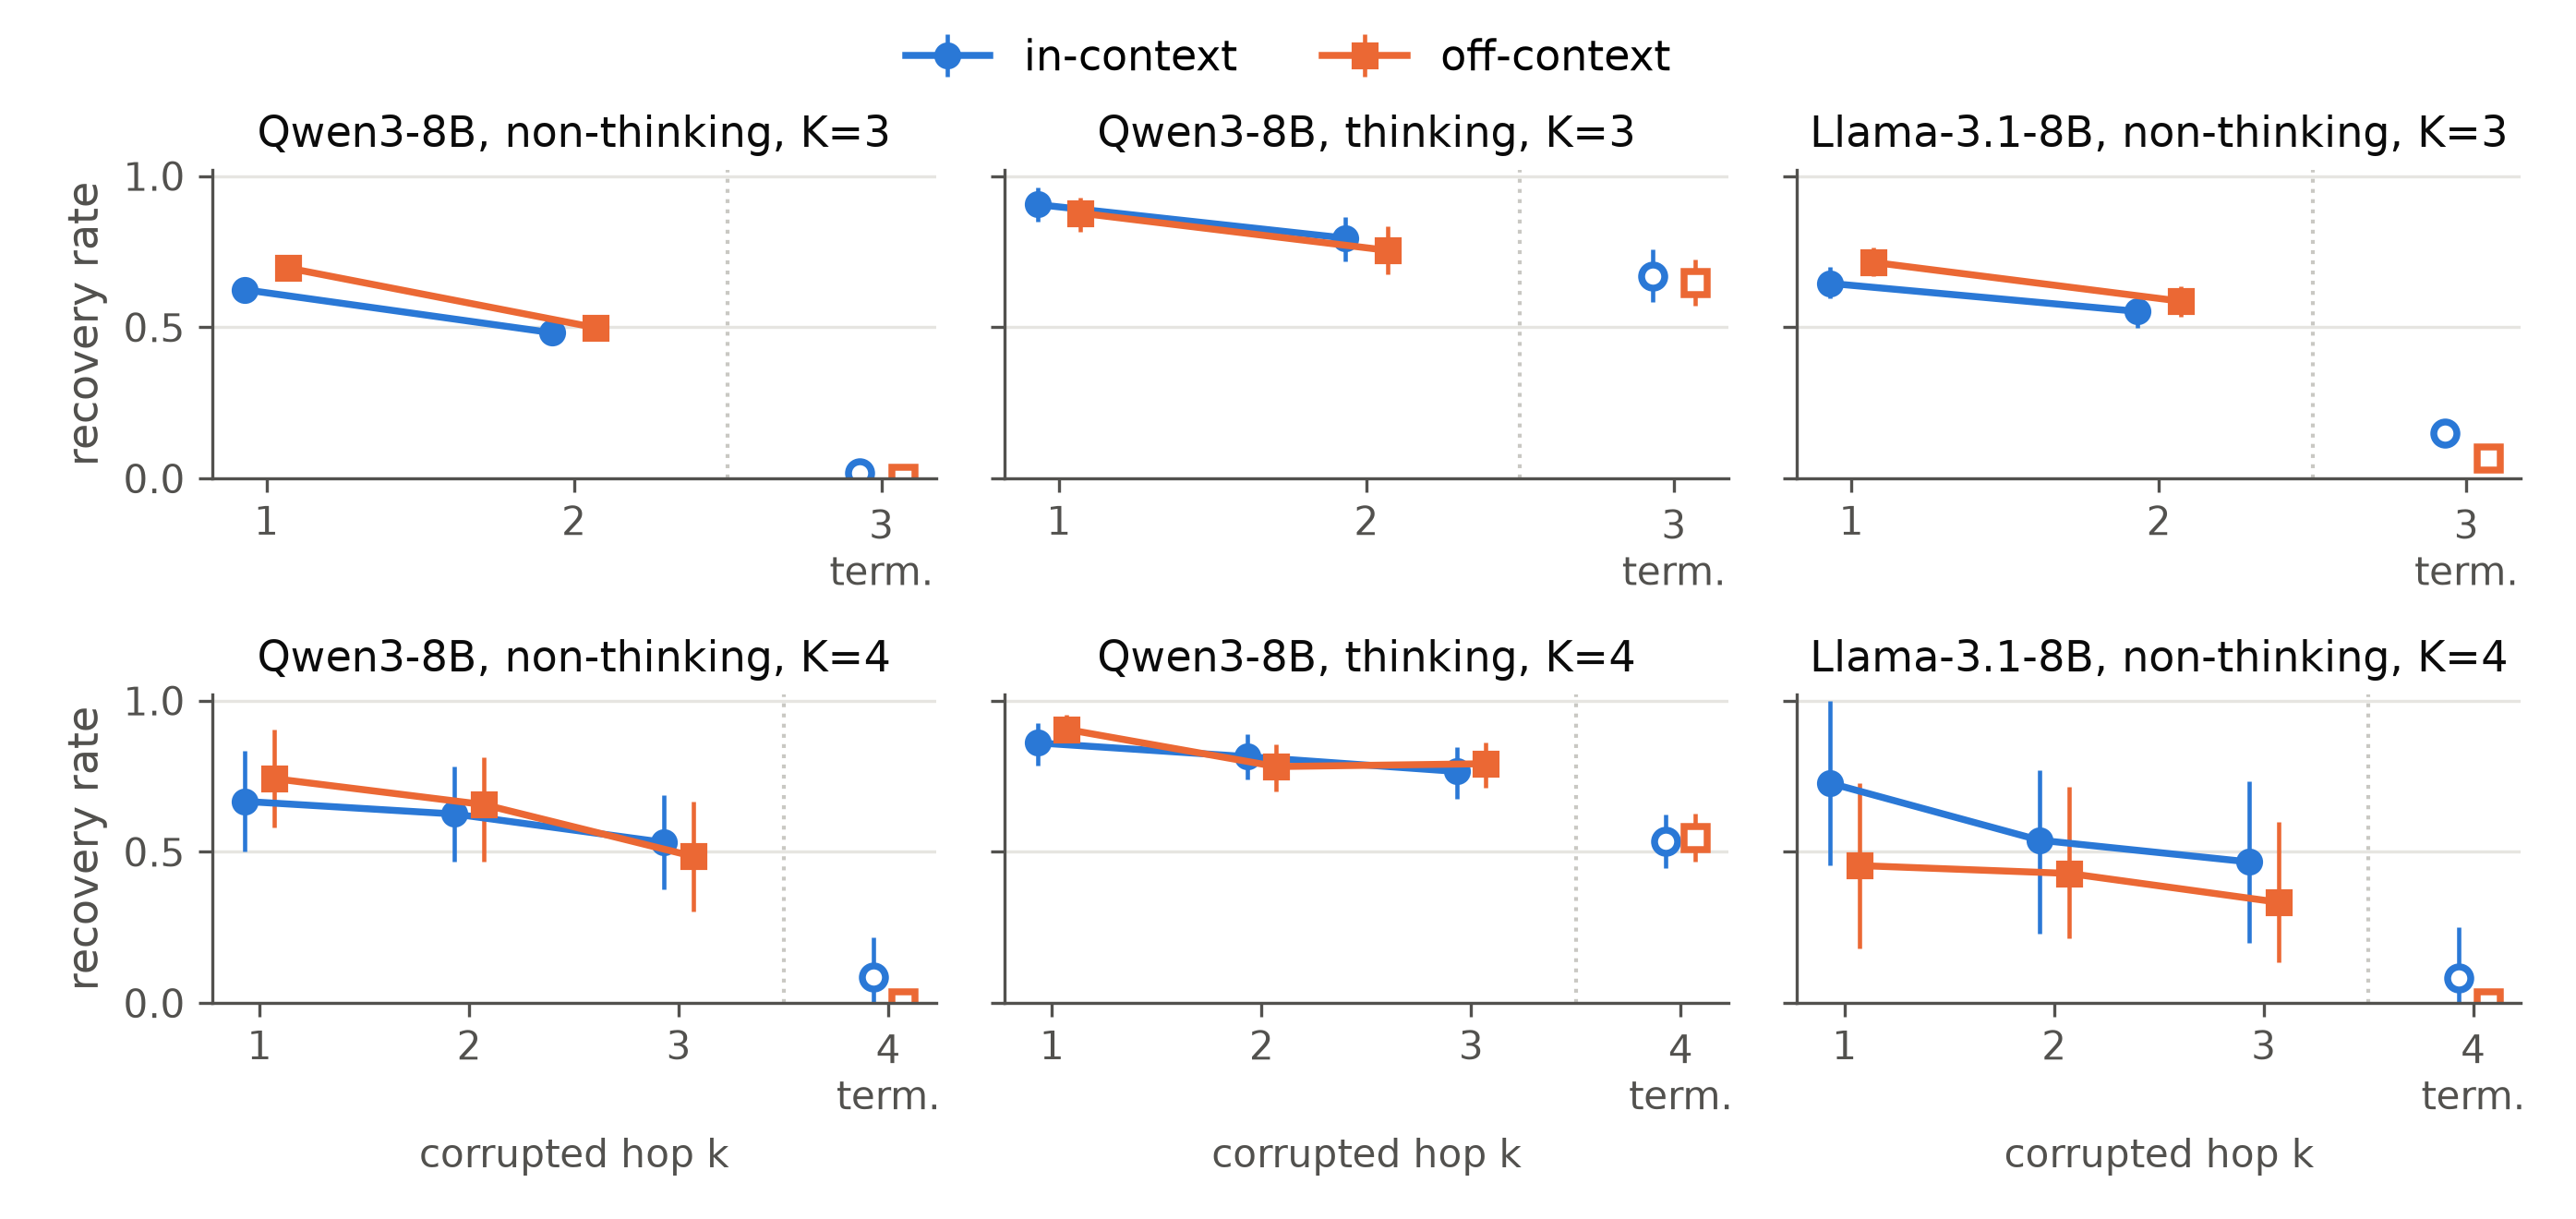
\includegraphics[width=0.92\textwidth]{figures/recovery_linear_paper.png}
\caption{Recovery rate by corrupted hop $k$ (linear chains; 95\% item-bootstrap CIs). Hollow markers: terminal hop, analyzed separately. Recovery falls from early to late intermediate hops in every panel and collapses at the terminal hop without thinking. The $K{=}4$ non-thinking panels rest on few items (33 for Qwen3, 15 for Llama).}
\label{fig:recovery}
\end{figure*}

\subsection{Resumption without an error (clean twins)}
\label{sec:res-twins}
Resuming from the model's own uncorrupted prefix succeeds at 96--100\% of intermediate hops for Qwen3 without thinking and 82--87\% for Llama ($K{=}3$). For Qwen3 with thinking it succeeds at only 68--86\% (terminal hop: 100\%), below the $\approx$90\% target set before the runs. An audit of all failing twins found no scoring error. Most leave the model's own chain at a later hop; about a fifth give the right entity at another granularity (``1991'' for \emph{December 25, 1991}). The cause in thinking mode is the prefix itself. With hop lines placed inside the think block, Qwen3 treats reasoning as finished: all 985 intermediate clean continuations contain only hop lines and a final answer, with a median of 110 generated tokens against 1{,}231 for an unprefixed resample. The prefill also costs accuracy in thinking mode (clean twin wrong and resample of the same item right in 183 cells vs.\ the reverse in 68; McNemar $p=2\times10^{-13}$) but not without thinking ($p=0.22$ for Qwen3). Thinking-mode $\RR$ is therefore measured on items the model can finish without further deliberation, and its continuations are short (Section~\ref{sec:res-thinking}).

\subsection{RQ1: Position of an intermediate error}
Late intermediate errors are recovered \emph{less} often than early ones, the opposite of H1 (Fig.~\ref{fig:recovery}, Table~\ref{tab:psi}). $\PSI$ is negative in all 12 model $\times$ mode $\times$ error type $\times K$ cells, and its CI excludes zero in 8; the four exceptions are the small four-hop non-thinking sets and one thinking cell whose CI reaches zero. The effect is clearest for Qwen3 without thinking at $K{=}3$, where recovery drops from 0.62 to 0.48 (in-context) and from 0.70 to 0.50 (off-context). In paired items, recovery at the early hop but not the late hop occurs 148 and 195 times, against 59 and 53 for the reverse (Holm-adjusted McNemar $p<10^{-8}$). Llama shows the same pattern at $K{=}3$ ($\PSI=-0.09$ and $-0.13$; McNemar $p_\text{Holm}=0.001$ for off-context). With thinking, $\PSI$ is $-0.09$ to $-0.12$, but its paired tests do not survive Holm adjustment (98--113 pairs per cell). No cell meets the $\pm$5\,pp equivalence criterion. The direction matches the late-stage fragility reported by ASCoT~\cite{ascot} and differs from the early-error findings of~\cite{vonrecum,jiamu}; Section~\ref{sec:res-rq2} suggests why.

\begin{table*}[t]
\centering
\caption{Position sensitivity $\PSI=\RR_\text{late}-\RR_\text{early}$ on intermediate hops (linear chains, 95\% item-bootstrap CIs). $n$: eligible linear items.}
\label{tab:psi}
\small
\setlength{\tabcolsep}{4pt}
\begin{tabular}{llrcc}
\toprule
 & $K$ & $n$ & in-context & off-context \\
\midrule
Qwen3, non-thinking & 3 & 763 & $-0.14$ [$-0.18$, $-0.10$] & $-0.20$ [$-0.24$, $-0.16$] \\
 & 4 & 33 & $-0.14$ [$-0.34$, $\phantom{-}0.07$] & $-0.26$ [$-0.47$, $-0.04$] \\
Qwen3, thinking & 3 & 147 & $-0.11$ [$-0.19$, $-0.04$] & $-0.12$ [$-0.21$, $-0.04$] \\
 & 4 & 154 & $-0.09$ [$-0.19$, $\phantom{-}0.00$] & $-0.11$ [$-0.20$, $-0.02$] \\
Llama-3.1, non-thinking & 3 & 438 & $-0.09$ [$-0.15$, $-0.03$] & $-0.13$ [$-0.19$, $-0.07$] \\
 & 4 & 15 & $-0.26$ [$-0.53$, $\phantom{-}0.00$] & $-0.12$ [$-0.39$, $\phantom{-}0.12$] \\
\bottomrule
\end{tabular}
\end{table*}

\textbf{Robustness to implausible planted values.}
\label{sec:res-tags}
Because many planted values are implausible (Section~\ref{sec:method}), we recomputed $\PSI$ by the type tag of the corrupted hop. Late-stage fragility is \emph{strongest} where planted values are cleanest. For PERSON, date and number values at $K{=}3$, $\PSI$ is $-0.31$ and $-0.37$ for Qwen3 without thinking and $-0.14$ and $-0.25$ for Llama. For places it is $-0.14$ to $-0.21$. It is near zero for ORG and NORP values, the least plausible. Implausible values thus dilute the position effect rather than produce it. The tag groups differ in which hops and items they cover (PERSON hops are mostly first hops), so we also tested the main contrast directly. The LLM rater judged a random sample of 200 cells from Qwen3 without thinking at $K{=}3$ (100 early, 100 late; outcomes hidden). Restricted to the 82 cells whose planted value was type-correct and plausible, recovery falls from 0.68 at the early hop to 0.37 at the late hop ($\PSI=-0.31$ [$-0.52$, $-0.11$]), against $-0.25$ [$-0.38$, $-0.11$] for all 200 cells. Implausible values are recovered somewhat more often at both hops (0.77 and 0.55).

\subsection{RQ2: Position or remaining steps?}
\label{sec:res-rq2}
On linear chains position and remaining steps move together, and the joint regression on those chains cannot split the effect between them (Table~\ref{tab:logit}; variance inflation factors 87 and 104). Three analyses separate them.
First, in branching items some hops at different positions have the same number of dependent later hops: in 3hop2, hops 1 and 2 both feed only hop 3. Within the same item, recovery at the later of two such positions minus the earlier one is $+0.05$ [$-0.02$, $0.12$] for Qwen3 without thinking (114 items) and $-0.01$ [$-0.10$, $0.08$] with thinking (42 items). Llama, however, still recovers less at the later position ($-0.12$ [$-0.22$, $-0.02$], 69 items). This need not be position as such. In 3hop2, an error at hop 1 is separated by an unrelated hop from the hop that uses it, whereas an error at hop 2 feeds that hop directly, so the distance to the consuming hop differs too.
Second, the matched-remaining contrasts on linear chains (same steps left, different absolute position) give differences of $-0.04$ to $+0.05$ for Qwen3 without thinking, although the four-hop cells hold only about 32 items.
Third, logistic models on all items that control for chain shape favour remaining steps over relative position for Qwen3 without thinking ($\Delta$AIC $=13.6$). In the joint model, remaining steps are significant ($\beta=0.75$, $p<0.001$) and relative position is not ($p=0.76$). For Llama and for Qwen3 with thinking, the two fit equally well ($\Delta$AIC $<2$).
For Qwen3, then, late-stage fragility follows the number of steps left after the error, not position itself. For Llama, the evidence leaves room for a position effect of its own.

\textbf{Why fewer remaining steps hurt (exploratory).} Reading the non-thinking continuations hop by hop shows the mechanism. After an error at hop $k$, we record the first later hop whose answer matches the gold hop again.
At $K{=}3$, Qwen3 gets back on track at the first hop after the error equally often for early and late errors (0.50 after hop 1, 0.51 after hop 2). These rates pool both error types and use the hop-matching rule, which is looser than the exact match behind $\RR$, so they differ slightly from the recovery rates above. Early errors recover more only because a second later hop catches a further 38\% of the remaining cases.
Llama is even more likely to get back on track at the first chance after a late error (0.58 vs.\ 0.39), but it too lacks the second chance, which catches 53\% for early errors.
Late errors are thus not harder to notice; they leave fewer hops on which to notice them.
The error usually propagates first. At $K{=}3$, Qwen3 writes the planted value into the next sub-question in 62--68\% of cells and Llama in 33--41\%. When it does, Qwen3 recovers in 46\% of cells, against 90\% when the next sub-question already uses the true value.
This may reconcile our result with the early-error findings of~\cite{vonrecum,jiamu}, though we have not tested it. In their math, science and logic tasks, later steps compute from earlier ones, so more remaining steps give an error more room to spread. Here, each later hop is looked up in the supplied paragraphs, so more remaining steps give the model more chances to re-ground.

\begin{table}[t]
\centering
\caption{Logistic regression of recovery on intermediate inject cells with a correct clean twin (linear chains; 5{,}670 cells, 1{,}177 items; item-clustered SEs). VIF: variance inflation factor. $^\dagger$Not interpretable: rel\_pos and remaining are near-collinear on linear chains; Section~\ref{sec:res-rq2} separates them.}
\label{tab:logit}
\small
\begin{tabular}{lrrrr}
\toprule
Term & $\beta$ & SE & $p$ & VIF \\
\midrule
\textcolor{gray}{rel\_pos$^\dagger$} & \textcolor{gray}{$-3.67$} & \textcolor{gray}{1.62} & \textcolor{gray}{0.023} & \textcolor{gray}{87} \\
\textcolor{gray}{remaining$^\dagger$} & \textcolor{gray}{$-0.58$} & \textcolor{gray}{0.52} & \textcolor{gray}{0.27} & \textcolor{gray}{104} \\
$K$ & $0.23$ & 0.30 & 0.44 & 11 \\
mode = thinking & $1.52$ & 0.32 & $<$0.001 & 13 \\
rel\_pos $\times$ thinking & $-0.24$ & 0.54 & 0.66 & 14 \\
off-context error & $0.15$ & 0.05 & 0.002 & 1.0 \\
item difficulty & $-1.12$ & 0.16 & $<$0.001 & 1.1 \\
model = Qwen3 & $-0.35$ & 0.09 & $<$0.001 & 1.2 \\
\bottomrule
\end{tabular}
\end{table}

\subsection{RQ3: The terminal step}
Errors at the terminal hop are almost never recovered without thinking: $\RR$ is 0.02 and 0.00 for Qwen3 (in-/off-context) and 0.15 and 0.07 for Llama, against 0.56--0.64 at intermediate hops of the same models. The models copy the corrupted last-hop answer into the final answer (Qwen3 adopts the planted value in 98--99\% of terminal cells, Llama in 75--88\%). With thinking, terminal recovery is 0.60 for both error types, still 0.22 below intermediate hops (CIs $-0.29$ to $-0.15$). Near-zero recovery here is expected, since the last hop's value is the answer and the model only has to copy it. Its importance lies in what pooling would do. Counting the terminal hop as ``late'', as designs that do not separate it effectively do, would multiply the apparent position effect by 2.3 to 3.2. For Qwen3 without thinking at $K{=}3$, $\PSI$ would be $-0.36$ and $-0.45$ instead of $-0.14$ and $-0.20$; for Llama, $-0.30$ and $-0.40$ instead of $-0.09$ and $-0.13$. ASCoT's largest accuracy drops came from exactly this step~\cite{ascot}.

\subsection{RQ4: Thinking mode}
\label{sec:res-thinking}
Recovery is higher in thinking mode at every hop: intermediate $\RR$ is 0.83 and 0.82 with thinking against 0.56 and 0.60 without (in-/off-context; mode $\beta=+1.52$, $p<0.001$). It does not change the shape: the relative position $\times$ mode interaction is small and not significant ($\beta=-0.24$, $p=0.66$), and late errors remain more harmful with thinking (Table~\ref{tab:psi}). Because eligibility differs between modes, we repeated the comparison on the 83 linear items eligible in both (63 three-hop, 20 four-hop). There, thinking still raises recovery on the same cells (intermediate $+0.24$ [0.17, 0.31]; terminal $+0.70$ [0.63, 0.78]), and the terminal hop stays below intermediate hops in both modes. Without thinking $\PSI$ stays negative ($K{=}3$: $-0.14$ and $-0.28$), but with thinking it shrinks to $0.00$ and $-0.10$ with CIs that include zero. The interaction remains non-significant ($p=0.34$) on this smaller set, so the shared items neither confirm nor rule out a change of shape.

These comparisons concern a thinking mode in which the model barely deliberates after the error (Section~\ref{sec:res-twins}): most recoveries happen when the model restates the chain after \texttt{</think>}, rewriting the corrupted hop with the correct entity. \tbd{think\_trace: error planted mid-thought in the model's own thinking trace; continuation length, clean-twin accuracy, $\RR$ and $\PSI$ vs.\ the summary-prefill condition. If continuations stay short, state the summary-prefill result as ``thinking format without post-error deliberation'' and move this to Limitations.}

\subsection{RQ5: Error type}
Off-context swaps, which nothing in the context supports, are recovered slightly more often than in-context distractors ($\beta=+0.15$, $p=0.002$; e.g., Qwen3 without thinking at $K{=}3$, $k{=}1$: 0.70 vs.\ 0.62). The difference is small next to the effects of position, the terminal hop and thinking. With thinking it is inconsistent in sign, and at Llama's terminal hop it reverses (0.15 in-context vs.\ 0.07 off-context).

\subsection{How recovery happens}
Recovery is almost always silent. A rule-based labeler calls a recovery \emph{explicit} if a doubt or correction marker (e.g., ``wait'', ``actually'', ``incorrect'', ``should be'') occurs in the same or the next sentence as the planted or the true hop value, and \emph{silent} otherwise. It marks none of Qwen3's non-thinking recoveries and 0.2\% of its thinking recoveries as explicit; Llama flags the error in 9\% of its intermediate-hop recoveries. Typically the model simply writes the correct entity in a later hop or in its restated chain, without commenting on the planted value. These labels are rule-based and were not validated by hand beyond spot checks.

\section{Limitations}
\textbf{Models.} We test two 8B models in 4-bit AWQ quantization. Larger or unquantized models may recover differently, and Fragile Thoughts~\cite{fragile} finds that scale partly protects against perturbations, though not for every error type.

\textbf{Planted errors.} Our errors are substituted values of the right type, not mistakes the model made itself. Natural errors may be correlated with item difficulty in ways planted ones are not. Type matching uses coarse spaCy tags, and in the audit only about half of the planted values were the right fine-grained type, with 41\% judged plausible by the LLM rater. The position effect is strongest among the cleanest values (Section~\ref{sec:res-tags}), and it holds on plausible values alone. Absolute recovery rates, however, are somewhat higher for implausible values, so they overstate recovery from realistic errors.

\textbf{Position and remaining steps.} On linear chains, position, remaining steps and chain length are tied together ($k$ + remaining $= K$). Branching items separate the two, but only for a minority of items (42--114 per model and mode). Four-hop items rarely pass eligibility without thinking (33 and 15 linear items), so the matched-remaining contrasts are underpowered. Branching items also differ from linear ones in ease, which our fit comparison controls for only through chain shape.

\textbf{Selection.} Eligibility keeps items that a model answers correctly along MuSiQue's decomposition and cannot answer closed-book (8--18\% of attempted items). Results therefore describe errors on solvable, gold-aligned items. Different modes are eligible on different items; the shared-item analysis covers only 83 linear items.

\textbf{Thinking-mode prefill.} With the hop summary prefilled inside the think block, Qwen3 stops deliberating: continuations are about 110 tokens, and clean twins succeed at only 68--86\% of intermediate hops. Our thinking-mode comparison is therefore between non-thinking generation and a thinking format with little deliberation after the error. Clean-twin conditioning further restricts it to items the model can finish without deliberating. \tbd{update after think\_trace.}

\textbf{Measurement.} Each cell has one sample, so item difficulty is binary. Exact match counts answers at a different granularity as wrong. Explicit and silent recovery labels are rule-based and were spot-checked only. The hop-by-hop recovery analysis relies on the same hop-matching rule as eligibility and covers non-thinking runs only. The thinking-mode cap of 4{,}096 tokens excluded 3\% of baselines.

\textbf{Data.} MuSiQue is built from English Wikipedia, which the models have likely seen in training. The closed-book filter removes only items a model answers from memory.

\section{Conclusion}
We planted errors at exact hop positions in models' own multi-hop reasoning and measured how often the models recover. In both models and both modes, late intermediate errors are recovered less often than early ones. This late-stage fragility holds even when the answer-producing hop is excluded; that hop is a separate case, almost never recovered without thinking. For Qwen3 it is explained by the number of steps left after the error rather than by position itself; for Llama the evidence is mixed. The next hop catches late errors at least as often as early ones, but late errors leave fewer hops on which to recover. This suggests that when each step is grounded in supplied evidence, an error is more dangerous the less reasoning remains after it. In our thinking condition, which leaves little deliberation after the error, recovery is higher but the position effect remains. Recovery is almost always silent. Our setting is narrow: two 4-bit 8B models, one dataset, substituted values, and supporting paragraphs in context. If these patterns hold beyond it, step-level checks in multi-step pipelines would do most good on late steps, and above all on the final step, rather than on the first. For studies that prefill reasoning models, they show that where the prefix is placed decides whether the model deliberates at all. \tbd{revise the thinking sentence after think\_trace.}

\bibliographystyle{IEEEtran}
\bibliography{refs}

\end{document}
